\documentclass{article}
\usepackage[utf8]{inputenc}
\usepackage[hidelinks]{hyperref}
\usepackage[spanish]{babel}
\usepackage[left=2cm,right=2cm,top=2cm,bottom=2cm]{geometry}
\usepackage{graphicx}
\usepackage{pdflscape}
\usepackage{listings}
\usepackage{cite} % Tidies up citation numbers.
\usepackage{url} % Provides better formatting of URLs.
\usepackage{booktabs} % Allows the use of \toprule, \midrule and \bottomrule in tables for horizontal lines
\usepackage{fancyhdr}
\usepackage[toc,page]{appendix}
\usepackage[dvipsnames]{xcolor}
\usepackage[stable]{footmisc}
\usepackage{amssymb}
\usepackage{float}



\lstset {
    frame = single,
    breaklines = true
}

\begin{document}
\begin{titlepage}
\title{\textbf{
    {\Huge Práctica 5: Minería de datos sobre un Data Mart}\\
    {\Large Almacenes y Minería de Datos}
}}
\author{
    Pedro Allué Tamargo (758267)
    \and
    Cristina Oriol García (755922)
    \and
    Alejandro Paricio García (761783)
}
\date{\today}
\clearpage\maketitle
\end{titlepage}

% Index
\tableofcontents

\newpage
\section{Introducción}

En la última práctica de la asignatura de minería de datos se pretende analizar los datos del data mart de vuelos creado y poblado en prácticas anteriores. El anterior contiene información acerca de vuelos en Estados Unidos que va a ser explotada con algunas de las distintas técnicas estudiadas en la asignatura. Entre ellas se encuentra la regresión paso a paso, las técnicas de agrupamiento, \textit{k-means} concretamente, el análisis de la varianza y las reglas de asociación. A continuación se detalla el uso dado a cada una de ellas y la información extraída de ellas, centrándose en estudiar los factores más influyentes y las causas del retraso de los vuelos.\\


\section{Regresión paso a paso}
\label{section:regPasoPaso}

Para la selección de los predictores que más influyen sobre el tiempo de retraso a la llegada se ha utilizado una regresión paso a paso. Al inicio se planteó como una regresión \textit{Lasso}, no obstante, con este método, podría ocurrir que la división de los $k$ posibles valores de la variable cualitativa en $k-1$ predictores llevase a que se incluyesen únicamente una parte de los anteriores, lo que no sería válido. Querríamos que, o bien el grupo de $k-1$ fuese incluido en su totalidad, o no fuese incluido, como ocurriría con una \textit{group lasso regression}.\\
La solución a este comportamiento ha sido la creación de un programa en \textit{R} que hiciera el proceso de regresión paso a paso utilizando las variables cuantitativas. El método de comparación de los predictores es mediante el \textit{Adjusted $R^2$}.\\

Los predictores que se han evaluado son: \textit{IDHORASALIDAREAL}, \textit{IDFECHASALIDA}, \textit{IDFECHALLEGADA}, \textit{IDHORALLEGADAREAL}, \textit{IDAEROLINEA}, \textit{IDAEROPUERTODESTINO}, \textit{IDAEROPUERTOORIGEN}, \textit{IDOPERADORA}. No se han utilizado los predictores \textit{NUMVUELO} ni \textit{IDAVION} ya que se ha estimado que es muy poco probable que sean influyentes a la hora de determinar del retraso. También se han desestimado por motivos técnicos, al ser factores con 5783 y 6653 niveles distintos no se obtenía resultado en un tiempo razonable.\\

El código utilizado para esta parte se puede encontrar en el Listing~\ref{listing:regresionPasoPasoR}. La salida de este código es la siguiente: 

\begin{lstlisting}
[...]
El mejor adjR2 es:  0.05026779NULL
[1] "IDHORASALIDAREAL"    "IDAEROPUERTOORIGEN"  "IDFECHALLEGADA"      "IDAEROPUERTODESTINO"
[5] "IDOPERADORA"         "IDHORALLEGADAREAL"   "IDFECHASALIDA"       "IDAEROLINEA"        
[1] 0.02484986 0.03490580 0.04194836 0.04635521 0.04860438 0.05005747 0.05021168 0.05026779
\end{lstlisting}


Se puede observar que el mejor \textit{Adjusted $R^2$} de la regresión paso a paso es \textit{0.05026779} que se corresponde con el modelo utilizando los predictores: \textit{IDHORASALIDAREAL, IDAEROPUERTOORIGEN, IDFECHALLEGADA, IDAEROPUERTODESTINO, IDOPERADORA, IDHORALLEGADAREAL, IDFECHASALIDA, IDAEROLINEA}. No obstante este valor para el \textit{Adjusted $R^2$} presenta un valor bastante pequeño. Se va a realizar un modelo de regresión lineal utilizando estos predictores. La salida del modelo de regresión lineal es la siguiente:

\begin{lstlisting}
Call:
lm(formula = TIEMPODERETRASOLLEGADA ~ IDHORASALIDAREAL + IDAEROPUERTOORIGEN + 
    IDFECHALLEGADA + IDAEROPUERTODESTINO + IDOPERADORA + IDHORALLEGADAREAL + 
    IDFECHASALIDA + IDAEROLINEA, data = vuelos.data)

Residuals:
    Min      1Q  Median      3Q     Max 
-725.44  -11.00   -5.13    1.13 1938.88 

Coefficients: (7 not defined because of singularities)
                           Estimate Std. Error t value Pr(>|t|)    
(Intercept)              -2.650e+00  7.392e+00  -0.358 0.719970    
IDHORASALIDAREAL2         1.085e+01  5.282e+00   2.053 0.040032 *  
IDHORASALIDAREAL3        -2.086e+00  6.267e+00  -0.333 0.739238    
IDHORASALIDAREAL4         4.180e+00  5.152e+00   0.811 0.417221    
IDHORASALIDAREAL5         1.286e+01  5.534e+00   2.324 0.020122 *  
IDHORASALIDAREAL6         1.177e+01  5.556e+00   2.118 0.034210 *  
IDHORASALIDAREAL7         6.904e+00  5.034e+00   1.372 0.170205    
IDHORASALIDAREAL8         5.895e+00  5.412e+00   1.089 0.276062    
IDHORASALIDAREAL9         1.420e+01  5.020e+00   2.830 0.004662 ** 
IDHORASALIDAREAL10        1.265e+01  5.026e+00   2.517 0.011839 * 
[...]
IDHORASALIDAREAL185       7.507e+00  5.057e+00   1.484 0.137680    
IDHORASALIDAREAL191       1.218e+01  5.081e+00   2.398 0.016484 *  
IDHORASALIDAREAL192       5.646e+00  5.660e+00   0.998 0.318511    
IDHORASALIDAREAL193       9.780e+00  5.330e+00   1.835 0.066554 .  
IDHORASALIDAREAL194      -1.574e+00  7.404e+00  -0.213 0.831612    
IDHORASALIDAREAL195       3.822e+00  5.199e+00   0.735 0.462240    
IDHORASALIDAREAL196       1.261e+01  5.093e+00   2.476 0.013303 *  
IDHORASALIDAREAL197       1.456e+01  5.544e+00   2.627 0.008619 ** 
IDHORASALIDAREAL198       1.870e+00  5.301e+00   0.353 0.724247    
IDHORASALIDAREAL199       1.074e+01  5.128e+00   2.094 0.036218 *  
IDHORASALIDAREAL200       1.902e-01  5.192e+00   0.037 0.970770    
 [ reached getOption("max.print") -- omitted 2576 rows ]
---
Signif. codes:  0 ‘***’ 0.001 ‘**’ 0.01 ‘*’ 0.05 ‘.’ 0.1 ‘ ’ 1

Residual standard error: 38.18 on 109217 degrees of freedom
Multiple R-squared:  0.07374,	Adjusted R-squared:  0.05027 
F-statistic: 3.141 on 2768 and 109217 DF,  p-value: < 2.2e-16
\end{lstlisting}

Se puede observar que la salida del modelo de regresión lineal muestra que este modelo explica solamente el \textit{7.374\%} de la varianza. También se puede observar que el \textit{p-valor} del \textit{F estadístico} es inferior a 0.05 y por lo tanto indica que alguno de los predictores tiene influencia sobre el modelo.\\

Por lo tanto se puede concluir con que el modelo con los predictores especificados es el que mejor \textit{Adjusted $R^2$} presenta en comparación, pero no explica gran parte de la varianza para el conjunto de datos.\\


\newpage
\section{K-means}

Se pretende clasificar los vuelos en tres grupos por retraso medio de los vuelos a la llegada en función de distintos factores. Antes de mostrar los resultados, ha de decidirse el formato de representación gráfica de los mismos. Como cada caso es en función de un único parámetro, lo más sencillo sería una representación unidimensional, pero de esa forma los datos no se podrían observar con facilidad. Por tanto, se ha optado por una representación bidimensional, en el que se mostrará una recta, ya que ambas coordenadas tendrán el mismo valor. De esta forma podrán visualizarse los resultados de forma sencilla. Además, los centroides también han sido representado, con color azul, pudiendo apreciarse cuáles son los puntos más cercanos a cada uno de ellos.\\


\subsection{Clasificación en función del aeropuerto de origen}

\begin{figure}[H]
    \centering
    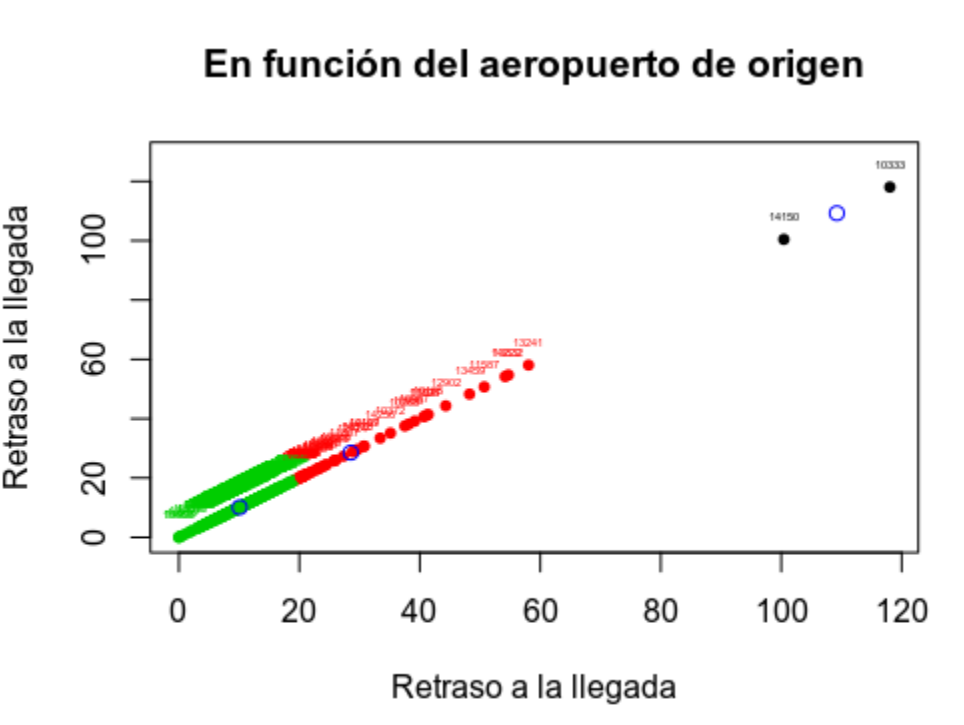
\includegraphics[width=0.7\columnwidth]{images/KMEANS/Origen.png}
    \caption{Kmeans, clasificación en función del aeropuerto de origen. }
    \label{fig:origen}
\end{figure}

En la imagen anterior se aprecian los identificadores de todos los aeropuertos de origen del data mart. Existen dos grupos muy poblados, el verde, con un retraso medio de llegada de los vuelos que parten de ellos menor a 20 minutos, y el rojo, cuyos aeropuertos oscilan entre 20 y 70 minutos de retraso medio. Finalmente, el tercer grupo consta de dos aeropuertos de los que parten vuelos con retraso mayor a 100 minutos, los que se corresponden con el aeropuerto de Alpena County Regional, Michigan (10333) y el de Pellston Regional Airport of Emmet County, Michigan (14150). Antes de extraer conclusiones, se van a visualizar el resto de clasificaciones.\\


\subsection{Clasificación en función del aeropuerto de destino}

\begin{figure}[H]
    \centering
    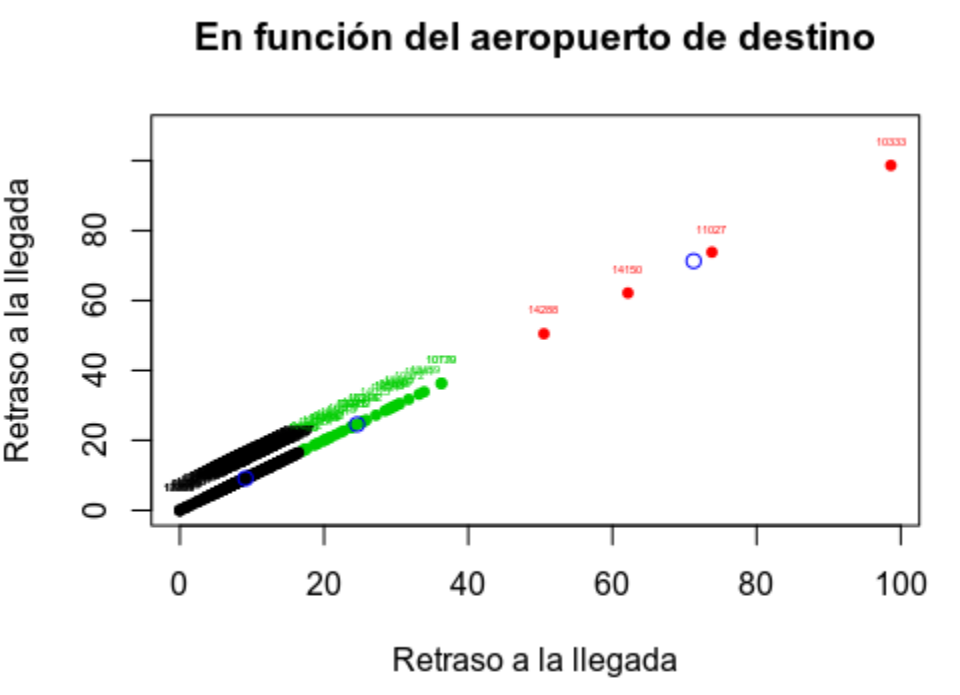
\includegraphics[width=0.7\columnwidth]{images/KMEANS/Destino.png}
    \caption{Kmeans, clasificación en función del aeropuerto de destino. }
    \label{fig:dest}
\end{figure}

De nuevo aparecen dos grupos bastante más poblado que el tercero, con unos rangos de retrasos a la llegada parecidos para los aeropuertos que los componen. Destaca el grupo rojo, en el que vuelven a aparecer los dos aeropuertos destacados en el apartado anterior, lo que parece ser coherente, a lo que se suman el North Central West Virginia, West Virginia (11027) y el aeropuerto Pueblo Memorial, Colorado (14288).\\


\subsection{Clasificación en función de la aerolínea}

\begin{figure}[H]
    \centering
    \includegraphics[width=0.7\columnwidth]{images/KMEANS/Aerolínea.png}
    \caption{Kmeans, clasificación en función de la aerolínea. }
    \label{fig:aero}
\end{figure}

Como puede observarse, el número de aerolíneas que han gestionado algún vuelo durante los días introducidos en el data mart es mucho menor que el de aeropuertos (al resto podría, por ejemplo, asignársele un retraso medio nulo). Debido a ello, controlan muchos más vuelos que un aeropuerto individualmente, lo que provoca que los grandes retrasos presentes en los aeropuertos anteriores sean mediados por otros vuelos con mucho menor retraso, provocando que la media de cada una de las aerolíneas sea mucho menor a la de los aeropuertos. Los tres grupos obtenidos dividen el espacio de aerolíneas en menos de 6 minutos de retraso medio, entre 6 y 9 minutos (aproximadamente), y aquellas con un retraso medio mayor a 9 minutos.

\newpage
\subsection{Clasificación en función de la matrícula}
 Debido a no contar con el modelo del avión, se ha decidido proceder con la matrícula de los mismos, siguiendo las indicaciones del profesor.
\begin{figure}[H]
    \centering
    \includegraphics[width=0.7\columnwidth]{images/KMEANS/Matrícula.png}
    \caption{Kmeans, clasificación en función de la matrícula del avión. }
    \label{fig:mat}
\end{figure}

Destaca a primera vista la gran cantidad de vehículos clasificados. Los tres centroides tienen asignados una gran cantidad de vehículos, pero es el grupo verde el que tiene un mayor rango de retrasos, destacando los dos aviones con más de 200 minutos de retraso medio (éstos solo han llevado a cabo un vuelo).

\subsection{Conclusión de las clasificaciones}
Tras haber llevado a cabo las clasificaciones anteriores, se puede extraer como conclusión que hay unos pocos aeropuertos que durante los días introducidos en el data mart han sufrido un retraso en los vuelos mucho mayor que otros. Especialmente relevantes son los aeropuertos de Alpena County Regional, Michigan y el de Pellston Regional Airport of Emmet County, Michigan, que aparecen en el grupo con más retraso tanto en los vuelos que salen de ellos, como en los que llegan. Eso parece indicar que algo ha perjudicado el rendimiento de ellos, al menos en los días tratados. El resto de aeropuertos se dividen en dos grupos, uno con retraso medio bajo, y otro con medio, lo que podría indicar que es necesario un análisis más exhaustivo en la gestión y rendimiento de los mismos, buscando un motivo de estos acontecimientos y, si es necesario, un resultado.\\

Por otro lado, también se pueden dividir en tres grupos las aerolíneas según su retraso, observando cuáles han funcionado mejor en media. No es suficiente para extraer una conclusión muy precisa, puesto que habría que tener en cuenta el número de vuelos gestionados por cada una, ya que una aerolínea ha podido gestionar un único vuelo con 20 minutos de retraso, mientras que otra retrasarse más de 20 minutos en uno de cada diez vuelos y en media funcionar mejor. Aún así, esta división puede servir para llevar a cabo una agrupación en tres grupos de las anteriores.\\

Por último se han clasificado los aviones, en función de su matrícula. De nuevo existen aviones que han llevado a cabo un único vuelo con mucho retraso, lo que puede tener distintos motivos a evaluar. Por ello habría que tener mucho cuidado a la hora de tomar decisiones teniendo en cuenta la anterior clasificación. Pese a ello, puede realizarse la clasificación pedida, como se observa en apartados anteriores.\\



\section{Análisis de la varianza}

Para el análisis acerca de que si los posibles retrasos pueden ser dependientes de las franjas horarias del horario de salida se ha utilizado un análisis de la varianza (\textit{ANOVA\footnote{\url{https://en.wikipedia.org/wiki/Analysis_of_variance}}}).\\

El primer para utilizar este método es la preparación de los datos. Se deben convertir las variables cualitativas que corresponden a los identificadores a 3 clases de variables. Estas variables se corresponden con las franjas horarias. La franja \textit{mañana} (M) se corresponde con la franja de \textit{7:00} a \textit{15:00} (no incluida). La franja \textit{tarde} (T) se corresponde con las horas entre las \textit{15:30} hasta las \textit{24:00} (no incluida). La franja \textit{noche} (N) se corresponde con la franja horaria restante \textit{24:00} hasta las \textit{7:00} (no incluida).\\

Tras la conversión de las variables cualitativas se va a proceder a la realización de un modelo de regresión lineal. El código encargado de realizar este modelo es el encontrado en el Listing~\ref{listing:anovaR}. La salida de este código es la siguiente:

\begin{lstlisting}
Call:
lm(formula = TIEMPODERETRASOLLEGADA ~ franja, data = vuelos.data.franjas)

Residuals:
    Min      1Q  Median      3Q     Max 
 -11.08  -10.08   -8.39   -4.15 2299.61 

Coefficients:
            Estimate Std. Error t value Pr(>|t|)    
(Intercept)  8.38800    0.08851   94.77   <2e-16 ***
franjaN     -4.23942    0.20997  -20.19   <2e-16 ***
franjaT      2.68714    0.13925   19.30   <2e-16 ***
---
Signif. codes:  0 ‘***’ 0.001 ‘**’ 0.01 ‘*’ 0.05 ‘.’ 0.1 ‘ ’ 1

Residual standard error: 39.29 on 373285 degrees of freedom
Multiple R-squared:  0.002846,	Adjusted R-squared:  0.00284 
F-statistic: 532.6 on 2 and 373285 DF,  p-value: < 2.2e-16

[1] "-----------------"
                Df    Sum Sq Mean Sq F value Pr(>F)    
franja           2   1644884  822442   532.6 <2e-16 ***
Residuals   373285 576374687    1544                   
---
Signif. codes:  0 ‘***’ 0.001 ‘**’ 0.01 ‘*’ 0.05 ‘.’ 0.1 ‘ ’ 1
[1] "-----------------"
  Tukey multiple comparisons of means
    95% family-wise confidence level

Fit: aov(formula = TIEMPODERETRASOLLEGADA ~ franja, data = vuelos.data.franjas)

$franja
         diff       lwr       upr p adj
N-M -4.239424 -4.731530 -3.747317     0
T-M  2.687140  2.360775  3.013506     0
T-N  6.926564  6.414101  7.439027     0
\end{lstlisting}



Se puede observar que la salida se compone de 3 secciones diferenciadas. La primera sección se corresponde con la salida de un modelo de regresión lineal. Se ha utilizado un modelo de regresión lineal para obtener una idea del comportamiento de la variable \textit{TIEMPODERETRASOLLEGADA} con respecto a la franja horaria en la hora de salida del vuelo. Se puede observar que el valor de \textit{Multiple R-squared} es \textit{0.002846}. Este valor es el que explica la proporción de la varianza explicada por el modelo. Al tener un valor bajo (\textit{0.2846\%}) indica que la variable \textit{franja} no explica una parte de la varianza que, a simple vista parece pequeña. También se puede observar que el \textit{p-valor} del \textit{F estadístico} es prácticamente 0 (\textit{2.2e-16}), esto implica que alguno de los predictores es influyente en el modelo.\\

La segunda sección se corresponde con la salida de un análisis de la varianza (\textit{aov}). Este análisis es una vista complementaria al modelo de regresión lineal anterior. Se puede observar que el valor del \textit{p-valor (Pr($>$F))} es inferior a 0.05 y por lo tanto indica que hay medias que son distintas.\\

La tercera sección se corresponde con la realización de un \textit{Test Turkey}. El objetivo de este test es adquirir información acerca de la diferencia de las medias de los factores de los estimadores. Se observa que el \textit{p adj} tiene un valor inferior a 0.05 y por lo tanto se puede deducir que las medias son distintas. Con este test se puede crear un diagrama de cajas (\textit{boxplot}) para comprobar gráficamente las diferencias entre las medias. El diagrama asociado muestra el intervalo de confianza de la diferencia de medias de cada uno de los factores de los predictores. Se puede comprobar que estas medias son distintas entre sí ya que ninguno de los intervalos contiene el 0. El diagrama de cajas se puede encontrar en la Figura~\ref{fig:testTukey}.\\

\begin{figure}[h!]
    \centering
    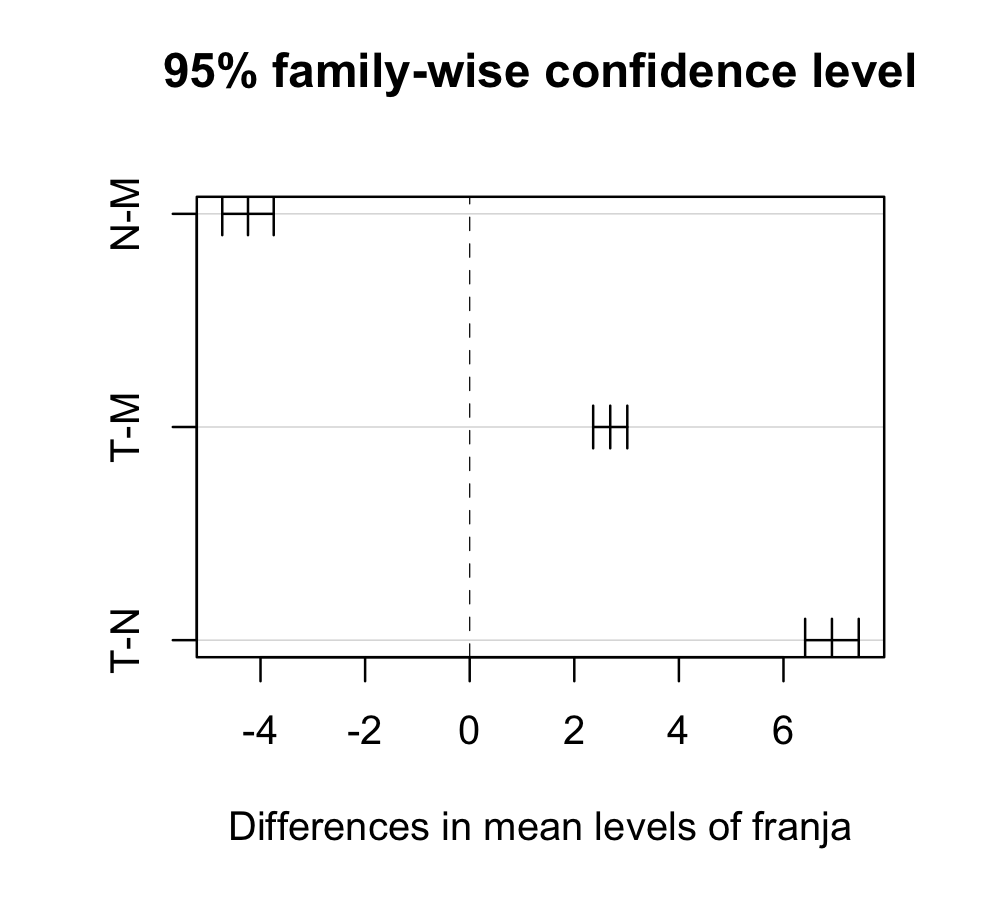
\includegraphics[width=0.7\columnwidth]{images/boxplot.png}
    \caption{Diagrama de comparación de medias del Test \textit{Tukey}}
    \label{fig:testTukey}
\end{figure}

Por lo tanto tras el estudio de lo anterior se puede concluir con que la franja horaria de la salida del vuelo no explica la varianza del retraso a la llegada. No obstante esto tiene sentido ya que solamente con la franja horaria de la hora de salida de los vuelos no se puede obtener una buena estimación del retraso a la llegada. Esto está respaldado por el apartado de regresión paso a paso (\ref{section:regPasoPaso}) que muestra que el mejor modelo con un único predictor es el correspondiente al utilizado para este análisis pero sin discretizar. Como se ha comentado anteriormente en la regresión paso a paso no se obtenían buenos resultados de predicción utilizando solamente este predictor.\\


\section{Reglas de asociación}

Hemos realizado un análisis de las reglas de asociación que podemos encontrar en en nuestros datos, intentando encontrar algún tipo de patrón que nos indique una relación entre nuestros distintos parámetros y los vuelos que llegan con retraso a su destino.\\

Para ello comenzamos preparando los datos para el análisis. Primero convertimos en factores las variables cualitativas \textit{IDHORASALIDAREAL, IDFECHASALIDA, IDAVION, IDFECHALLEGADA, IDHORALLEGADAREAL, IDAEROLINEA, IDAEROPUERTODESTINO, IDAEROPUERTOORIGEN y IDOPERADORA}. A continuación tenemos que transformar la variable \textit{TIEMPODERETRASOLLEGADA}, esta nos da el tiempo de retraso de los vuelos en las llegada en minutos, para ello realizamos siete grupos clasificando los retrasos en \textit{Hasta10, Hasta20, Hasta30, Hasta40, Hasta50, Hasta1hora, Más1hora}, grupos de diez minutos hasta llegar a una hora que se clasifican todos como más de una hora. A continuación nos queda realiza grupos con las horas de salida de los vuelos, para ello hemos tenido que leer otro fichero csv que relaciona los id con la hora en formato \textit{hora:minutos}, de este fichero nos quedamos este segundo parámetro haciendo tres grupos \textit{Mañana, Tarde y Noche} y lo unimos a los parámetros originales. Teniendo ya todos transformados los transformamos en transacciones. \\

A continuación con \textit{apriori} se realiza un análisis sobre los datos para encontrar información respecto al soporte y decidir cuál puede ser el valor correcto a utilizar. El resultado obtenido es:\\
\begin{lstlisting}
     Min.   1st Qu.    Median      Mean   3rd Qu.      Max. 
0.0000027 0.0001232 0.0001795 0.0012226 0.0002465 0.4643278 
\end{lstlisting}
\subsection{Apriori}
Para un primer análisis con apriori se ha utilizado la mediana como minsup y una confianza de 0'6. Con lo que se han generado un total de \textit{195866} reglas. Sin embargo si comprobamos aquellas reglas en las que estabamos interesados, las que en el consecuente contienen \textit{TIEMPODERETRASOLLEGADA} y observamos que únicamente tenemos 6, las siguientes ordenadas por lift:
\begin{lstlisting}
        lhs                            rhs                                    support confidence     coverage     lift count
[1] {IDFECHALLEGADA=23,                                                                                                 
     IDAEROLINEA=537,                                                                                                   
     IDAEROPUERTODESTINO=12953,                                                                                         
     HORAMINUTOS24HORAS=Noche}  => {TIEMPODERETRASOLLEGADA=Más1hora} 0.0001151926  1.0000000 0.0001151926 31.76108    43
[2] {IDFECHASALIDA=23,                                                                                                  
     IDAEROLINEA=537,                                                                                                   
     IDAEROPUERTODESTINO=12953,                                                                                         
     HORAMINUTOS24HORAS=Noche}  => {TIEMPODERETRASOLLEGADA=Más1hora} 0.0001151926  1.0000000 0.0001151926 31.76108    43
[3] {IDFECHASALIDA=23,                                                                                                  
     IDFECHALLEGADA=23,                                                                                                 
     IDAEROLINEA=537,                                                                                                   
     IDAEROPUERTODESTINO=12953,                                                                                         
     HORAMINUTOS24HORAS=Noche}  => {TIEMPODERETRASOLLEGADA=Más1hora} 0.0001151926  1.0000000 0.0001151926 31.76108    43
[4] {IDFECHALLEGADA=23,                                                                                                 
     IDAEROPUERTODESTINO=12953,                                                                                         
     HORAMINUTOS24HORAS=Noche}  => {TIEMPODERETRASOLLEGADA=Más1hora} 0.0001821650  0.7727273 0.0002357429 24.54265    68
[5] {IDFECHASALIDA=23,                                                                                                  
     IDAEROPUERTODESTINO=12953,                                                                                         
     HORAMINUTOS24HORAS=Noche}  => {TIEMPODERETRASOLLEGADA=Más1hora} 0.0001821650  0.7727273 0.0002357429 24.54265    68
[6] {IDFECHASALIDA=23,                                                                                                  
     IDFECHALLEGADA=23,                                                                                                 
     IDAEROPUERTODESTINO=12953,                                                                                         
     HORAMINUTOS24HORAS=Noche}  => {TIEMPODERETRASOLLEGADA=Más1hora} 0.0001821650  0.7727273 0.0002357429 24.54265    68
\end{lstlisting}

Como se puede observar los valores son sospechosos ya que estarían haciendo referencia al mismo vuelo con distintos parámetros en la regla. 
La primera regla correspondería a:
\begin{lstlisting}
                  2020-01-16, Maersk Air I/S, LaGuardia','NY','New York', Noche => Retraso de más de una hora
\end{lstlisting}

Que únicamente encontremos seis reglas, referentes al mismo vuelo puede ser debido a que tenemos un alto número de parámetros que generan de por si reglas entre ellos ya que muchos de estos parámetros están relacionados entre sí, como las aerolíneas y los aviones lo que provoca que aumente el soporte bajando el de las reglas que realmente nos interesan. Por ello realizo un segundo análisis con un minsup de 0.00005 con lo que obtenemos 24 reglas que contienen el tiempo de retraso en el consecuente. Aquí se muestran las diez primeras ordenadas por lift:
\begin{lstlisting}
             lhs                            rhs                                    support confidence     coverage     lift count
[1]  {IDFECHALLEGADA=23,                                                                                                 
      IDAEROLINEA=537,                                                                                                   
      IDAEROPUERTODESTINO=12953,                                                                                         
      HORAMINUTOS24HORAS=Noche}  => {TIEMPODERETRASOLLEGADA=Más1hora} 1.151926e-04  1.0000000 1.151926e-04 31.76108    43
[2]  {IDFECHASALIDA=23,                                                                                                  
      IDAEROLINEA=537,                                                                                                   
      IDAEROPUERTODESTINO=12953,                                                                                         
      HORAMINUTOS24HORAS=Noche}  => {TIEMPODERETRASOLLEGADA=Más1hora} 1.151926e-04  1.0000000 1.151926e-04 31.76108    43
[3]  {IDFECHASALIDA=23,                                                                                                  
      IDFECHALLEGADA=23,                                                                                                 
      IDAEROLINEA=537,                                                                                                   
      IDAEROPUERTODESTINO=12953,                                                                                         
      HORAMINUTOS24HORAS=Noche}  => {TIEMPODERETRASOLLEGADA=Más1hora} 1.151926e-04  1.0000000 1.151926e-04 31.76108    43
[4]  {IDFECHALLEGADA=23,                                                                                                 
      IDAEROPUERTODESTINO=12953,                                                                                         
      HORAMINUTOS24HORAS=Noche}  => {TIEMPODERETRASOLLEGADA=Más1hora} 1.821650e-04  0.7727273 2.357429e-04 24.54265    68
[5]  {IDFECHASALIDA=23,                                                                                                  
      IDAEROPUERTODESTINO=12953,                                                                                         
      HORAMINUTOS24HORAS=Noche}  => {TIEMPODERETRASOLLEGADA=Más1hora} 1.821650e-04  0.7727273 2.357429e-04 24.54265    68
[6]  {IDFECHASALIDA=23,                                                                                                  
      IDFECHALLEGADA=23,                                                                                                 
      IDAEROPUERTODESTINO=12953,                                                                                         
      HORAMINUTOS24HORAS=Noche}  => {TIEMPODERETRASOLLEGADA=Más1hora} 1.821650e-04  0.7727273 2.357429e-04 24.54265    68
[7]  {IDFECHASALIDA=21,                                                                                                  
      IDFECHALLEGADA=21,                                                                                                 
      IDAEROPUERTODESTINO=12478,                                                                                         
      HORAMINUTOS24HORAS=Noche}  => {TIEMPODERETRASOLLEGADA=Más1hora} 5.893573e-05  0.6875000 8.572470e-05 21.83574    22
[8]  {IDFECHALLEGADA=21,                                                                                                 
      IDAEROPUERTODESTINO=12478,                                                                                         
      HORAMINUTOS24HORAS=Noche}  => {TIEMPODERETRASOLLEGADA=Más1hora} 5.893573e-05  0.6666667 8.840359e-05 21.17405    22
[9]  {IDFECHALLEGADA=23,                                                                                                 
      IDAEROLINEA=537,                                                                                                   
      IDAEROPUERTOORIGEN=12953,                                                                                          
      HORAMINUTOS24HORAS=Noche}  => {TIEMPODERETRASOLLEGADA=Más1hora} 7.768800e-05  0.6590909 1.178715e-04 20.93344    29
[10] {IDFECHASALIDA=23,                                                                                                  
      IDAEROLINEA=537,                                                                                                   
      IDAEROPUERTOORIGEN=12953,                                                                                          
      HORAMINUTOS24HORAS=Noche}  => {TIEMPODERETRASOLLEGADA=Más1hora} 7.768800e-05  0.6590909 1.178715e-04 20.93344    29
\end{lstlisting}
La primera regla volvería a coindicir con la mostrada anteriormente:
\begin{lstlisting}
                  2020-01-16, Maersk Air I/S, LaGuardia','NY','New York', Noche => Retraso de más de una hora
\end{lstlisting}
Lo que observamos de estos resultados es que las reglas con más lift son las que se refieren a un tiempo de retraso mayor de una hora y sigue pareciendo que algunas de ellas acaban señalando el mismo de distitnas formas, en el antecedente encontramos un alto número de variables lo que posiblemente signifique que se está refiriendo a un vuelo concreto. Por ello procedemos a restringir el número de factores a tener en cuenta a 4. Con minsup=0.00005 obtenemos ocho reglas que contienen el retraso:
\begin{lstlisting}
            lhs                            rhs                                    support confidence     coverage     lift count
[1] {IDFECHALLEGADA=23,                                                                                                 
     IDAEROPUERTODESTINO=12953,                                                                                         
     HORAMINUTOS24HORAS=Noche}  => {TIEMPODERETRASOLLEGADA=Más1hora} 1.821650e-04  0.7727273 2.357429e-04 24.54265    68
[2] {IDFECHASALIDA=23,                                                                                                  
     IDAEROPUERTODESTINO=12953,                                                                                         
     HORAMINUTOS24HORAS=Noche}  => {TIEMPODERETRASOLLEGADA=Más1hora} 1.821650e-04  0.7727273 2.357429e-04 24.54265    68
[3] {IDFECHALLEGADA=23,                                                                                                 
     IDAEROPUERTODESTINO=12953,                                                                                         
     IDOPERADORA=537}           => {TIEMPODERETRASOLLEGADA=Más1hora} 7.500911e-05  0.6363636 1.178715e-04 20.21160    28
[4] {IDFECHASALIDA=23,                                                                                                  
     IDAEROPUERTODESTINO=12953,                                                                                         
     IDOPERADORA=537}           => {TIEMPODERETRASOLLEGADA=Más1hora} 7.500911e-05  0.6363636 1.178715e-04 20.21160    28
[5] {IDFECHASALIDA=21,                                                                                                  
     IDAEROPUERTODESTINO=12478,                                                                                         
     HORAMINUTOS24HORAS=Noche}  => {TIEMPODERETRASOLLEGADA=Más1hora} 5.893573e-05  0.6285714 9.376139e-05 19.96411    22
[6] {IDFECHALLEGADA=21,                                                                                                 
     IDAEROPUERTODESTINO=12478,                                                                                         
     HORAMINUTOS24HORAS=Noche}  => {TIEMPODERETRASOLLEGADA=Más1hora} 5.893573e-05  0.6666667 8.840359e-05 21.17405    22
[7] {IDFECHALLEGADA=23,                                                                                                 
     IDAEROPUERTODESTINO=12953,                                                                                         
     IDOPERADORA=167}           => {TIEMPODERETRASOLLEGADA=Más1hora} 5.893573e-05  0.6111111 9.644028e-05 19.40955    22
[8] {IDFECHASALIDA=23,                                                                                                  
     IDAEROPUERTODESTINO=12953,                                                                                         
     IDOPERADORA=167}           => {TIEMPODERETRASOLLEGADA=Más1hora} 5.893573e-05  0.6111111 9.644028e-05 19.40955    22
     
\end{lstlisting}
Siguen siendo pocas reglas y seguimos teniendo el problema de que parecen referir únicamente a un vuelo y varias de ellas al mismo, si bajamos el support a 0.00002 obtenemos 33 reglas, las diez primeras ordenadas por support:
\begin{lstlisting}
              lhs                            rhs                                    support confidence     coverage      lift count
[1]  {IDFECHALLEGADA=23,                                                                                                  
      IDAEROPUERTODESTINO=12953,                                                                                          
      HORAMINUTOS24HORAS=Noche}  => {TIEMPODERETRASOLLEGADA=Más1hora} 1.821650e-04  0.7727273 2.357429e-04 24.542654    68
[2]  {IDFECHASALIDA=23,                                                                                                   
      IDAEROPUERTODESTINO=12953,                                                                                          
      HORAMINUTOS24HORAS=Noche}  => {TIEMPODERETRASOLLEGADA=Más1hora} 1.821650e-04  0.7727273 2.357429e-04 24.542654    68
[3]  {IDFECHALLEGADA=23,                                                                                                  
      IDAEROPUERTODESTINO=12953,                                                                                          
      IDOPERADORA=537}           => {TIEMPODERETRASOLLEGADA=Más1hora} 7.500911e-05  0.6363636 1.178715e-04 20.211598    28
[4]  {IDFECHASALIDA=23,                                                                                                   
      IDAEROPUERTODESTINO=12953,                                                                                          
      IDOPERADORA=537}           => {TIEMPODERETRASOLLEGADA=Más1hora} 7.500911e-05  0.6363636 1.178715e-04 20.211598    28
[5]  {IDFECHASALIDA=21,                                                                                                   
      IDAEROPUERTODESTINO=12478,                                                                                          
      HORAMINUTOS24HORAS=Noche}  => {TIEMPODERETRASOLLEGADA=Más1hora} 5.893573e-05  0.6285714 9.376139e-05 19.964109    22
[6]  {IDFECHALLEGADA=21,                                                                                                  
      IDAEROPUERTODESTINO=12478,                                                                                          
      HORAMINUTOS24HORAS=Noche}  => {TIEMPODERETRASOLLEGADA=Más1hora} 5.893573e-05  0.6666667 8.840359e-05 21.174055    22
[7]  {IDFECHALLEGADA=23,                                                                                                  
      IDAEROPUERTODESTINO=12953,                                                                                          
      IDOPERADORA=167}           => {TIEMPODERETRASOLLEGADA=Más1hora} 5.893573e-05  0.6111111 9.644028e-05 19.409550    22
[8]  {IDFECHASALIDA=23,                                                                                                   
      IDAEROPUERTODESTINO=12953,                                                                                          
      IDOPERADORA=167}           => {TIEMPODERETRASOLLEGADA=Más1hora} 5.893573e-05  0.6111111 9.644028e-05 19.409550    22
[9]  {IDFECHALLEGADA=3,                                                                                                   
      IDAEROPUERTOORIGEN=12889,                                                                                           
      IDOPERADORA=537}           => {TIEMPODERETRASOLLEGADA=Hasta10}  4.018345e-05  0.6521739 6.161462e-05  6.109433    15
[10] {IDFECHASALIDA=35,                                                                                                   
      IDAEROPUERTOORIGEN=12889,                                                                                           
      IDOPERADORA=537}           => {TIEMPODERETRASOLLEGADA=Hasta10}  4.018345e-05  0.6521739 6.161462e-05  6.109433    15
\end{lstlisting}

Ahora obtenemos reglas que parecen ser un poco distintas entre sí. 

\subsection{Eclat}
Otro análisis de reglas realizado ha sido utilizando \textit{Eclat} en vez de \textit{Apriori}. Para ello realizamos un primer conjunto de itemsets frecuentes con minsup=0.0001 y buscamos reglas con confianza de 0.6, en ellas obtenemos 6 reglas que contienen el tiempo de retraso e el consecuente:
\begin{lstlisting}
                  lhs                            rhs                                    support confidence     lift itemset
[1] {IDFECHASALIDA=23,                                                                                       
     IDFECHALLEGADA=23,                                                                                      
     IDAEROPUERTODESTINO=12953,                                                                              
     HORAMINUTOS24HORAS=Noche}  => {TIEMPODERETRASOLLEGADA=Más1hora} 0.0001821650  0.7727273 24.54265  127229
[2] {IDFECHALLEGADA=23,                                                                                      
     IDAEROPUERTODESTINO=12953,                                                                              
     HORAMINUTOS24HORAS=Noche}  => {TIEMPODERETRASOLLEGADA=Más1hora} 0.0001821650  0.7727273 24.54265  127244
[3] {IDFECHASALIDA=23,                                                                                       
     IDAEROPUERTODESTINO=12953,                                                                              
     HORAMINUTOS24HORAS=Noche}  => {TIEMPODERETRASOLLEGADA=Más1hora} 0.0001821650  0.7727273 24.54265  127322
[4] {IDFECHASALIDA=23,                                                                                       
     IDFECHALLEGADA=23,                                                                                      
     IDAEROLINEA=537,                                                                                        
     IDAEROPUERTODESTINO=12953,                                                                              
     HORAMINUTOS24HORAS=Noche}  => {TIEMPODERETRASOLLEGADA=Más1hora} 0.0001151926  1.0000000 31.76108  127227
[5] {IDFECHALLEGADA=23,                                                                                      
     IDAEROLINEA=537,                                                                                        
     IDAEROPUERTODESTINO=12953,                                                                              
     HORAMINUTOS24HORAS=Noche}  => {TIEMPODERETRASOLLEGADA=Más1hora} 0.0001151926  1.0000000 31.76108  127242
[6] {IDFECHASALIDA=23,                                                                                       
     IDAEROLINEA=537,                                                                                        
     IDAEROPUERTODESTINO=12953,                                                                              
     HORAMINUTOS24HORAS=Noche}  => {TIEMPODERETRASOLLEGADA=Más1hora} 0.0001151926  1.0000000 31.76108  127320
\end{lstlisting}

Con estas reglas nos sucede lo mismo que pasaba con las generadas \textit{apriori}. Parecen apuntar a un único vuelo y ser las seis iguales con distintos parámetros. 


\subsection{Itemsets frecuentes maximales y cerrados}

El último análisis realizado lo llevamos a cabo calculando un conjunto de itemsets frecuentes maximales con apriori, y otro conjunto con itemsets frecuentes cerrados también con apriori, minsup=0.00005 y de estos obtenemos las reglas con una confianza de 0.6, de estas 5 contienen el retraso:
\begin{lstlisting}
                  lhs                            rhs                                    support confidence     lift itemset
[1] {IDFECHASALIDA=23,                                                                                       
     IDFECHALLEGADA=23,                                                                                      
     IDAEROLINEA=537,                                                                                        
     IDAEROPUERTODESTINO=12953,                                                                              
     HORAMINUTOS24HORAS=Noche}  => {TIEMPODERETRASOLLEGADA=Más1hora} 1.151926e-04  1.0000000 31.76108   49454
[2] {IDFECHASALIDA=23,                                                                                       
     IDFECHALLEGADA=23,                                                                                      
     IDAEROLINEA=537,                                                                                        
     IDAEROPUERTOORIGEN=12953,                                                                               
     HORAMINUTOS24HORAS=Noche}  => {TIEMPODERETRASOLLEGADA=Más1hora} 7.768800e-05  0.6590909 20.93344   49361
[3] {IDFECHASALIDA=23,                                                                                       
     IDFECHALLEGADA=23,                                                                                      
     IDAEROLINEA=537,                                                                                        
     IDAEROPUERTODESTINO=12953,                                                                              
     IDOPERADORA=537}           => {TIEMPODERETRASOLLEGADA=Más1hora} 7.500911e-05  0.6363636 20.21160   49453
[4] {IDFECHASALIDA=21,                                                                                       
     IDFECHALLEGADA=21,                                                                                      
     IDAEROPUERTODESTINO=12478,                                                                              
     HORAMINUTOS24HORAS=Noche}  => {TIEMPODERETRASOLLEGADA=Más1hora} 5.893573e-05  0.6875000 21.83574   36978
[5] {IDFECHASALIDA=23,                                                                                       
     IDFECHALLEGADA=23,                                                                                      
     IDAEROLINEA=537,                                                                                        
     IDAEROPUERTODESTINO=12953,                                                                              
     IDOPERADORA=167}           => {TIEMPODERETRASOLLEGADA=Más1hora} 5.893573e-05  0.6111111 19.40955   49452
\end{lstlisting}


\newpage
\section{Conclusiones}

Se han estudiado los datos utilizando múltiples técnicas de minería de datos. Las técnicas utilizadas pasan la regresión paso a paso para evaluar qué predictores son influyentes en los datos para determinar el retraso. También se utilizan métodos de agrupamiento como \textit{K-Means} para intentar agrupar los datos en función del retraso con respecto a variables como el aeropuerto de origen, la aerolínea o la matrícula del avión. Otro análisis realizado ha sido el estudio de la varianza presentada en los datos del retraso con respecto a la franja horaria de la salida. Esta franja se encontraba dividida de forma predeterminada en tres grupos: mañana, tarde, noche.
Con respecto a las reglas de asociación se puede observar que no es fácil encontrar patrones para formar reglas que nos expliquen el retraso, siendo este el parámetro sujeto de nuestro estudio, aún incluso bajando ampliamente el support no conseguimos encontrar reglas suficientemente generales que nos den buenos resultados de este análisis.\\

\subsection{Control de esfuerzos}
\begin{itemize}
    \item Pedro Allué Tamargo: regresión paso a paso, análisis de la varianza y la correspondiente memoria. Conclusión de la memoria. 
        \begin{itemize}
            \item Horas invertidas: 8h
        \end{itemize}
    \item Cristina Oriol García: Construcción de las reglas de asociación y la correspondiente memoria. 
        \begin{itemize}
            \item Horas invertidas: 8h
        \end{itemize}
    \item Alejandro Paricio García: kmeans y la correspondiente memoria. Ayuda con el planteamiento regresión paso a paso. Introducción y estructura de la memoria.
        \begin{itemize}
            \item Horas invertidas: 7h
        \end{itemize}
\end{itemize}


% Anexo de código
\newpage
\section*{Anexo 1: Códigos}

\subsection*{Código de la regresión paso a paso}

\lstinputlisting[language=R, label={listing:regresionPasoPasoR}, caption={Código de la regresión paso a paso}]{listings/regresionPasoPaso.R}


\subsection*{Código del análisis de la varianza}

\lstinputlisting[language=R, label={listing:anovaR}, caption={Código del análisis de la varianza}]{listings/anova.R}


% Bibliografía
\newpage
\addcontentsline{toc}{section}{Referencias}
\bibliographystyle{unsrt}
\bibliography{bibliografia.bib}

\end{document}